
\documentclass{bredelebeamer}
\usepackage{verbatim}
\usepackage{tikz}
\usetikzlibrary{mindmap,shadows}
\usepackage[spanish,es-nodecimaldot]{babel}
\usepackage{ragged2e}
\usepackage{etoolbox}
\usepackage{lipsum}

\usepackage{subcaption}

% Information boxes
\newcommand*{\info}[4][16.3]{%
  \node [ annotation, #3, scale=0.85, text width = #1em,
          inner sep = 2mm ] at (#2) {%
  \list{$\bullet$}{\topsep=0pt\itemsep=0pt\parsep=0pt
    \parskip=0pt\labelwidth=8pt\leftmargin=8pt
    \itemindent=0pt\labelsep=2pt}%
    #4
  \endlist
  };
}

\title[Proyecto PAP]{Proyecto de Aplicaci\'on Profesional}
\subtitle{Modelos de predici\'on en empresas y gobierno
mediante aprendizaje estad\'istico. \\
Profesor: Dr. P\'ablo D\'avalos de la Pe\~na}

\author{%
    \textbf{Juan Francisco Mu\~noz Elguez\'abal} \\
    Alumno Ingenier\'ia Financiera \\
    \textcolor{blue}{\texttt{IF149833@iteso.mx}} \vspace{5pt} \\
    \textbf{Rodrigo Ledesma Elorriaga} \\
    Alumno Ingenier\'ia Financiera \\
    \textcolor{blue}{\texttt{IF149833@iteso.mx}} \vspace{5pt} \\
    \textbf{Zurisadai Velazquez Manzanero} \\
    Alumno Ingenier\'ia Financiera \\
    \textcolor{blue}{\texttt{IF149833@iteso.mx}} \vspace{5pt}}

\institute[ITESO]
{  }

\date{3.Diciembre.2015}

\begin{document}

% -- ----------------------------------------------------------------------------- -- %
% -- ---------------------------------------------------------- Portada Lamina (1) -- %
% -- ----------------------------------------------------------------------------- -- %

\begin{frame}{}
  \titlepage
\end{frame}

% -- ----------------------------------------------------------------------------- -- %
% -- ----------------------------------------------------- Proyecto PAP Lamina (2) -- %
% -- ----------------------------------------------------------------------------- -- %

\begin{frame}{Mapa de contenidos}

\begin{figure}[H]
\centering
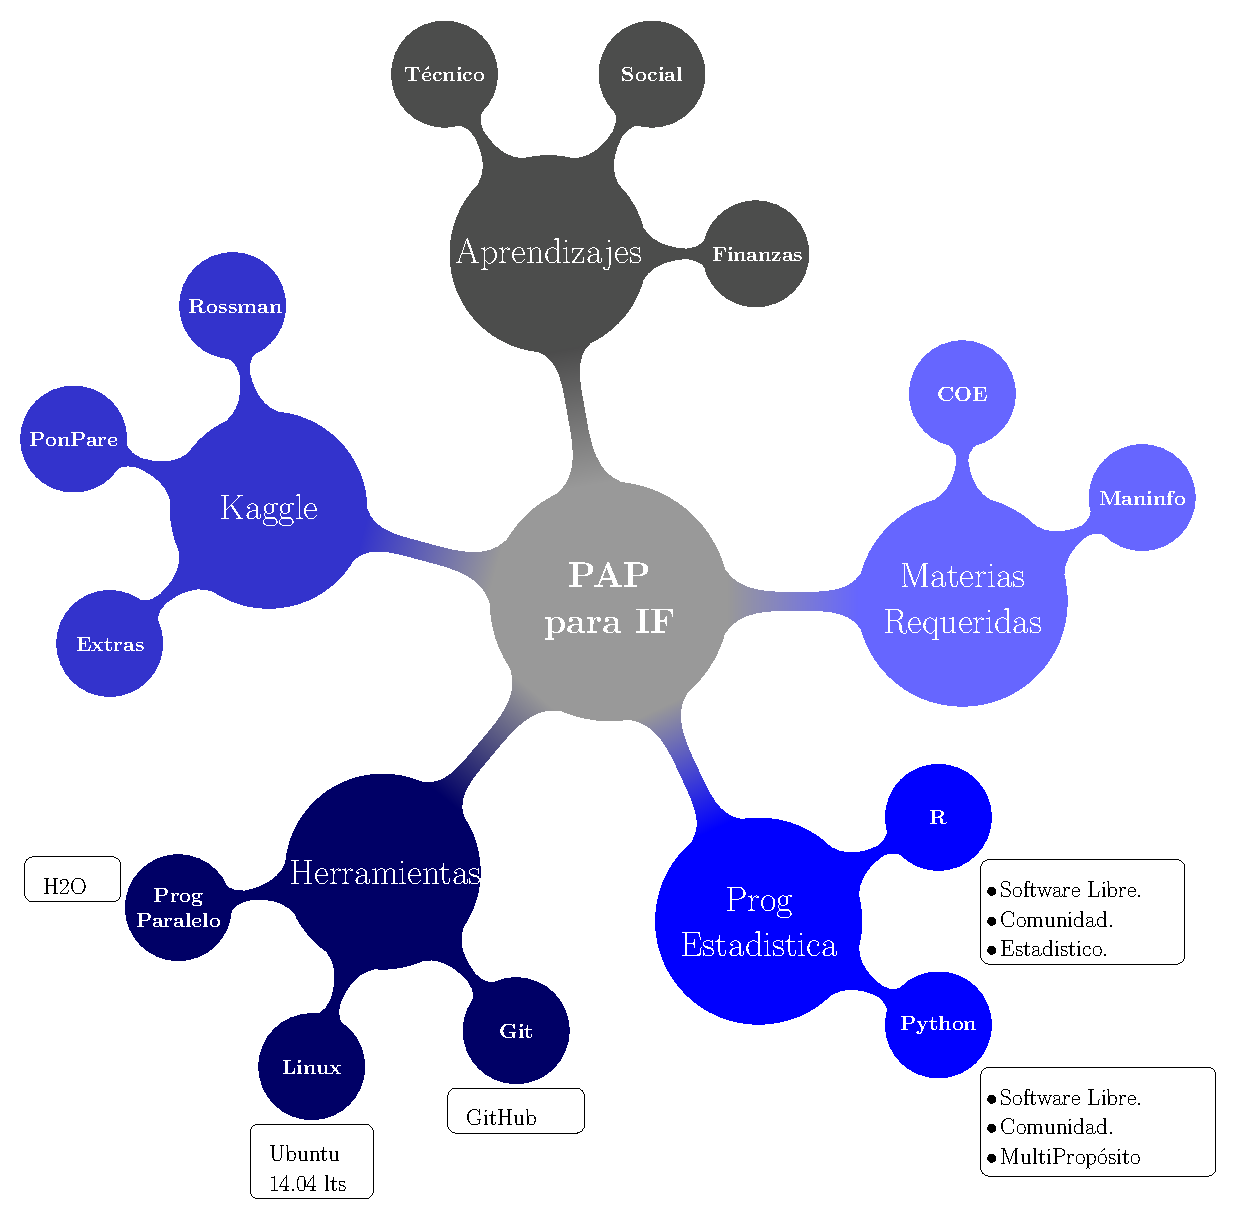
\includegraphics[scale=.36]{MindMap.pdf}
\end{figure}

\end{frame}

% -- ----------------------------------------------------------------------------- -- %
% -- --------------------------------------- Contenidos de Presentacion Lamina (3) -- %
% -- ----------------------------------------------------------------------------- -- %

\begin{frame}{Un Proyecto de Aplicaci\'on Profesional}

\begin{itemize}

  \item \textbf{Creditos Aprobados:} 70\% antes de inscribirlo.
  \item \textbf{Materia Requerida 1:} Manejo de informac\'on y datos num\'ericos.
  \item \textbf{Materia Requerida 2:} Comunicaci\'on oral y escr\'ita.
  \item \textbf{Especiales:} Pre-requisitos de Carrera y Pre-requisitos de Proyecto.

\end{itemize}

\vspace{1cm}

\textit{Fuente:}  \textit{Video Tutorial PAP - canal oficial Pap Iteso} \\
\textcolor{blue}{\href{https://www.youtube.com/watch?v=LFYJOpu97m8}{https://www.youtube.com/watch?v=LFYJOpu97m8}}

\end{frame}

% -- ----------------------------------------------------------------------------- -- %
% -- ----------------------------------------------- Kaggle y Machine Learning (4) -- %
% -- ----------------------------------------------------------------------------- -- %

\begin{frame}{Ciencia de datos en PAP}

\justifying

\textbf{Colaboraci\'on \textcolor{blue}{KUESKI}}: \textit{En espera} \\
\vspace{.2cm}

Seguridad de informaci\'on comprometida.

\vspace{.75cm}
  
\textbf{Colaboraci\'on \textcolor{blue}{ITESO}}: \textit{En espera} \\
\vspace{.2cm}

Seguridad de informaci\'y beneficio contrario a la naturaleza del PAP.

\vspace{.75cm}

\textbf{Aprendizaje competitivo \textcolor{blue}{KAGGLE}}: \textit{Utilizado} \\
\vspace{.2cm}

Un sitio donde se publican retos competitivos, para
recompensa y/o incluso reclutamiento a trav\'es de an\'alisis de datos para 
clasificaci\'on y predicci\'on. Frecuentado por cient\'ificos de datos profesionales
y por organizaciones como \textit{Netflix}, \textit{Airbnb},
\textit{Walmart}, \textit{Hillary Clinton's Emails}, entre otros.

\end{frame}

% -- ----------------------------------------------------------------------------- -- %
% -- -------------------------- Herramientas Computacionales Utilizadas Lamina (6) -- %
% -- ----------------------------------------------------------------------------- -- %

\begin{frame}{Herramientas Computacionales I: GITHUB en LINUX}

\begin{figure}
\centering
\begin{subfigure}{.5\textwidth}
  \centering
  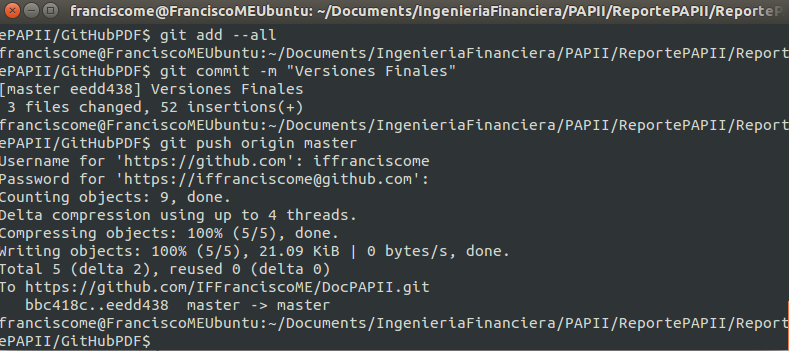
\includegraphics[width=1.1\linewidth]{images/GitHubLINUX.png}
  \caption{GitHub en LINUX}
\end{subfigure}%
\begin{subfigure}{.5\textwidth}
  \centering
  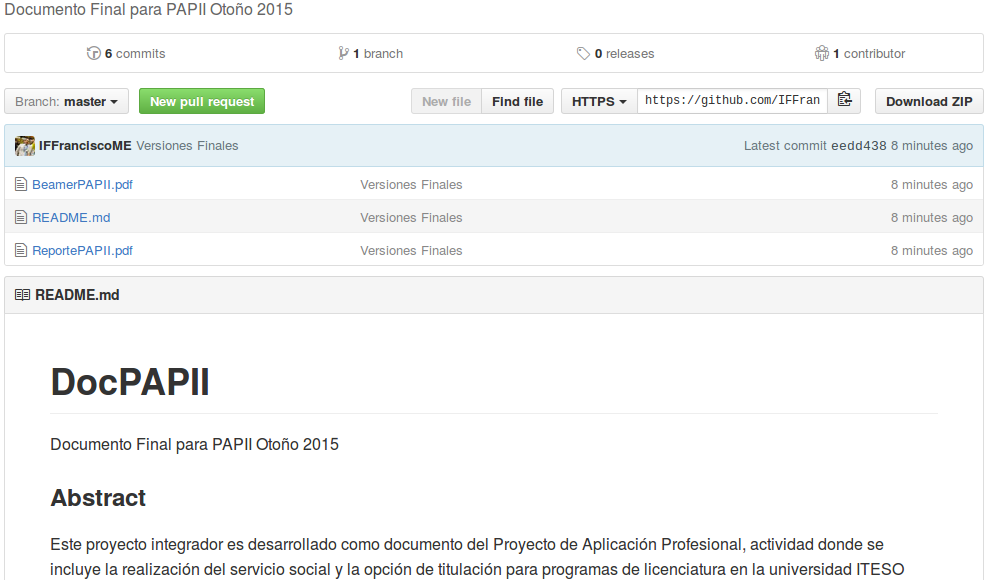
\includegraphics[width=.85\linewidth]{images/GitHubWEB.png}
  \caption{GitHub en WEB}
\end{subfigure}
\end{figure}

\begin{figure}[H]
\centering
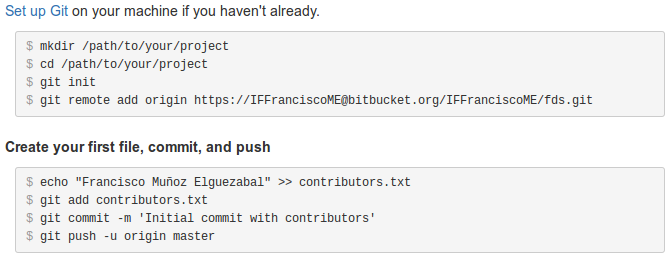
\includegraphics[scale=.34]{images/SetupGit.png}
\end{figure}


\end{frame}

% -- ----------------------------------------------------------------------------- -- %
% -- -------------------------- Herramientas Computacionales Utilizadas Lamina (7) -- %
% -- ----------------------------------------------------------------------------- -- %

\begin{frame}{Herramientas Computacionales I: Lenguajes, IDEs, S.O.}

Se utiliz\'o una computadora Toshiba U940 i5 8gb, 1.7Mhz. Las herramientas computacionales
instaladas en esta y que fueron utilizadas durante el transcurso del proyecto fueron las
siguientes:

\begin{block}{Lenguajes de Programaci\'on}
Versi\'on de \textit{R}: \\
Versi\'on de \textit{Python}:
\end{block}

\begin{block}{IDEs (Integrated Development Environment)}
Versi\'on \textit{RStudio}: \\
Versi\'on \textit{Pycharm}:
\end{block}

\begin{block}{Sistema Operativo:}
Linux: Ubuntu 14.04 LTS
\end{block}

\end{frame}

% -- ----------------------------------------------------------------------------- -- %
% -- ------------------------------------------ Analisis exploratorio I Lamina (8) -- %
% -- ----------------------------------------------------------------------------- -- %

\begin{frame}{Herramientas Computacionales II: Librerias Especiales}

\begin{itemize}

  \item \textbf{R}: \textit{data.table} Paqueter\'ia para tratamiento de \textit{BigData}
  \item \textbf{Software}: Cluster de procesamiento en paralelo Online/Local \textit{H2O}
  
\end{itemize}

\begin{figure}
\centering
\begin{subfigure}{.5\textwidth}
  \centering
  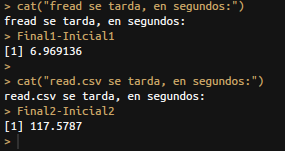
\includegraphics[width=.9\linewidth]{images/freadVSreadcsv.png}
  \caption{fread VS readcsv}
\end{subfigure}%
\begin{subfigure}{.5\textwidth}
  \centering
  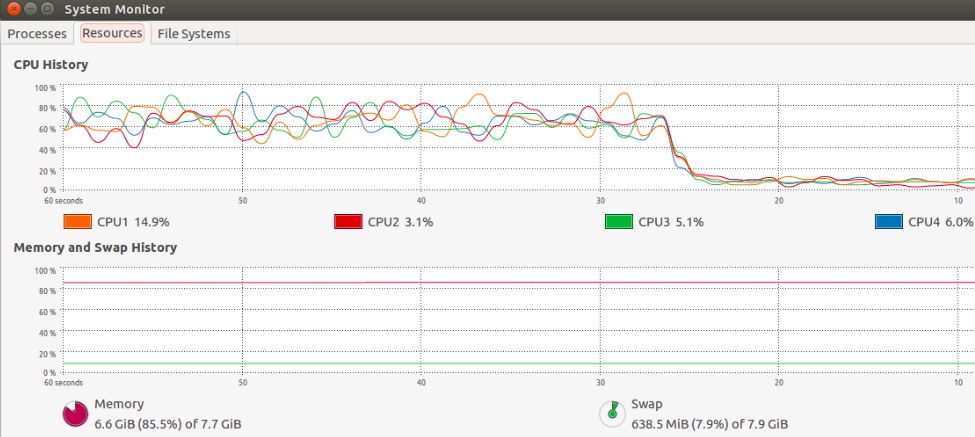
\includegraphics[width=1.1\linewidth]{images/H2O.png}
  \caption{4 Procesadores y 90\% Ram}
\end{subfigure}

\vspace{1cm}

\caption{Recursos en Lectura y Procesamiento de datos}
\end{figure}

\end{frame}

% -- ----------------------------------------------------------------------------- -- %
% -- ------------------------------------------ Analisis exploratorio I Lamina (8) -- %
% -- ----------------------------------------------------------------------------- -- %

\begin{frame}{Herramientas Computacionales III: Librerias Especiales}

\begin{figure}
\centering
\begin{subfigure}{.5\textwidth}
  \centering
  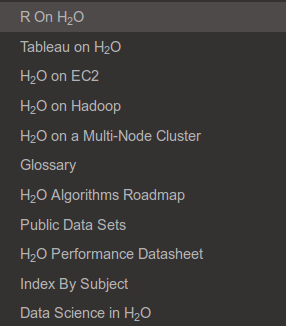
\includegraphics[width=.75\linewidth]{images/H2OServices.png}
  \caption{H2O Integraciones}
\end{subfigure}%
\begin{subfigure}{.5\textwidth}
  \centering
  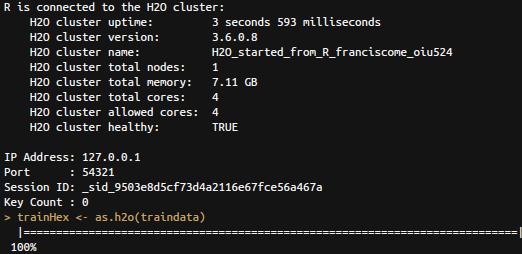
\includegraphics[width=1.1\linewidth]{images/H2OServices2.png}
  \caption{En m\'aquina local}
\end{subfigure}

\vspace{.75cm}

\caption{Recursos en Lectura y Procesamiento de datos}
\end{figure}

\end{frame}


% -- ----------------------------------------------------------------------------- -- %
% -- ------------------------------------------ Analisis exploratorio I Lamina (9) -- %
% -- ----------------------------------------------------------------------------- -- %

\begin{frame}{APLICACI\'ON: Ciencia de Datos para Series de Tiempo I}

Predicci\'on para series de tiempo financieras mediante la implementaci\'on y
clasificaci\'on de estudios de an\'alisis t\'ecnico.

\vspace{.05cm}

\begin{figure}
\centering
\begin{subfigure}{.5\textwidth}
  \centering
  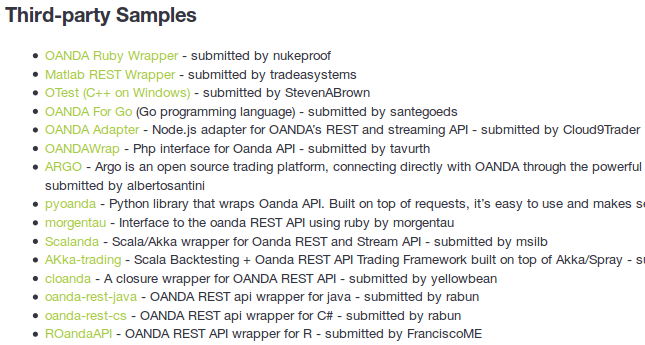
\includegraphics[width=.95\linewidth]{images/ROanda.png}
  \caption{API en R}
\end{subfigure}%
\begin{subfigure}{.5\textwidth}
  \centering
  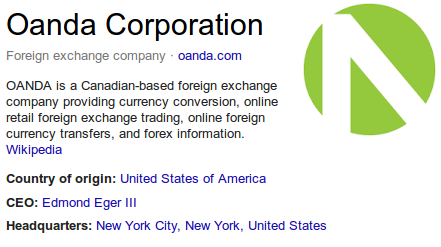
\includegraphics[width=.9\linewidth]{images/ROanda1.png}
  \caption{Broker Online de Forex}
\end{subfigure}

\vspace{.75cm}

\caption{Recursos en Lectura y Procesamiento de datos}
\end{figure}

\end{frame}

% -- ----------------------------------------------------------------------------- -- %
% -- ------------------------------------------ Analisis exploratorio I Lamina (9) -- %
% -- ----------------------------------------------------------------------------- -- %

\begin{frame}{APLICACI\'ON: Ciencia de Datos para Series de Tiempo II}

C\'odigo b\'asico para utilizar la API de \textit{ROanda} y obtener informaci\'on del
mercado en tiempo real, hist\'orica, grautita y de 120 instrumentos financieros.

\begin{figure}[H]
\centering
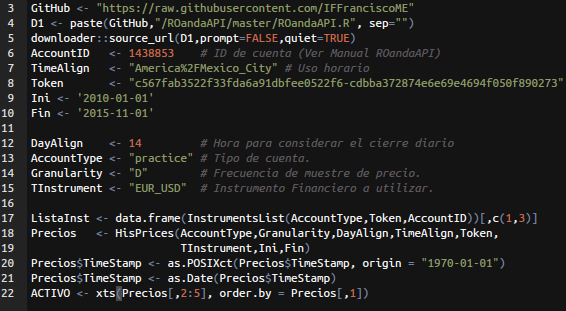
\includegraphics[scale=.4]{images/ROanda2.png}
\end{figure}



\end{frame}

% -- ----------------------------------------------------------------------------- -- %
% -- ------------------------------------------ Analisis exploratorio I Lamina (9) -- %
% -- ----------------------------------------------------------------------------- -- %

\begin{frame}{APLICACI\'ON: Ciencia de Datos para Series de Tiempo III}

Realizar ciencia de datos para observaciones no secuenciales o distintas de series de
tiempo es lo que aprendimos, pero tambi\'en a trasladar t\'ecnicas y metodolog\'ias al
caso de series de tiempo financieras, como el caso de realizar los siguiente:

\begin{itemize}

  \item CrossValidation K-Fold para \textit{series de tiempo} ?

\end{itemize}

\boitegrise{
Fold <- trunc(length(Tdata.train[,1])/10) \\
Train1 <- Tdata.train[1:Fold,] \\ 
Train2 <- Tdata.train[1:(Fold*2),] \\
Train3 <- Tdata.train[1:(Fold*3),] \\
Train4 <- Tdata.train[1:(Fold*4),] \\
Train5 <- Tdata.train[1:(Fold*5),] \\
Train6 <- Tdata.train[1:(Fold*6),] \\
Train7 <- Tdata.train[1:(Fold*7),] \\
Train8 <- Tdata.train[1:(Fold*8),] \\
Train9 <- Tdata.train[1:(Fold*9),] \\
Train10 <- Tdata.train[1:(Fold*10),]
}

\end{frame}

% -- ----------------------------------------------------------------------------- -- %
% -- ------------------------------------------ Analisis exploratorio I Lamina (10) -- %
% -- ----------------------------------------------------------------------------- -- %

\begin{frame}{An\'alisis T\'ecnico y Ciencia de Datos.}

\begin{figure}
\centering
\begin{subfigure}{.5\textwidth}
  \centering
  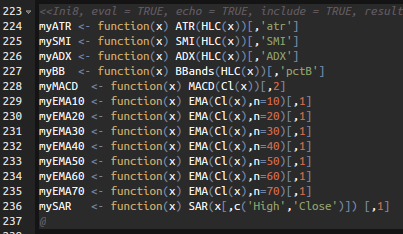
\includegraphics[width=.9\linewidth]{images/Codigo1.png}
  \caption{Funciones Gen\'ericas}
\end{subfigure}%
\begin{subfigure}{.5\textwidth}
  \centering
  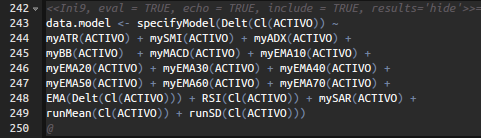
\includegraphics[width=1.1\linewidth]{images/Codigo2.png}
  \caption{Modelo General}
\end{subfigure}

\vspace{.75cm}

\caption{An\'alisis t\'ecnico y Machine Learning I}
\end{figure}

\end{frame}

% -- ----------------------------------------------------------------------------- -- %
% -- ------------------------------------------ Propuesta de modelos I Lamina (11) -- %
% -- ----------------------------------------------------------------------------- -- %

\begin{frame}{An\'alisis exploratorio}

Se establecieron los criterios de toma de postura de la siguiente manera:

\begin{itemize}

  \item $ x >= -0.005 $ - "hold" 
  \item $ x <= 0.005 $ - "hold" 
  \item $ x >   0.005$ - "buy" 
  \item $ x <  -0.005$ - "sell"

\end{itemize}

\begin{figure}
\centering
\begin{subfigure}{.5\textwidth}
  \centering
  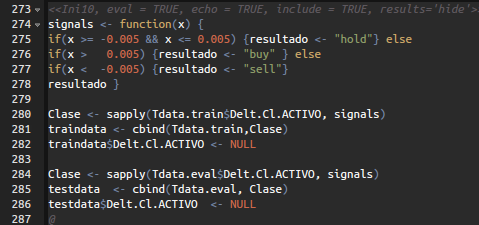
\includegraphics[width=.9\linewidth]{images/Codigo3.png}
  \caption{Consideraci\'on para se\~nales }
\end{subfigure}%
\begin{subfigure}{.5\textwidth}
  \centering
  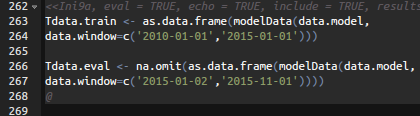
\includegraphics[width=1.1\linewidth]{images/Codigo4.png}
  \caption{Evaluaci\'on y Prueba}
\end{subfigure}
\end{figure}

  
\end{frame}

% -- ----------------------------------------------------------------------------- -- %
% -- ------------------------------------------ Analisis exploratorio I Lamina (9) -- %
% -- ----------------------------------------------------------------------------- -- %

\begin{frame}{Modelos de Machine Learning}

Se ajustaron dos modelos, el primero fue el visto en el PAP, \textit{Random Forest},
utilizando la librer\'ia de R con el mismo nombre. El segundo a manera de comparaci\'on
fue una red neuronal del tipo perceptr\'on multicapa.

\begin{figure}
\centering
\begin{subfigure}{.5\textwidth}
  \centering
  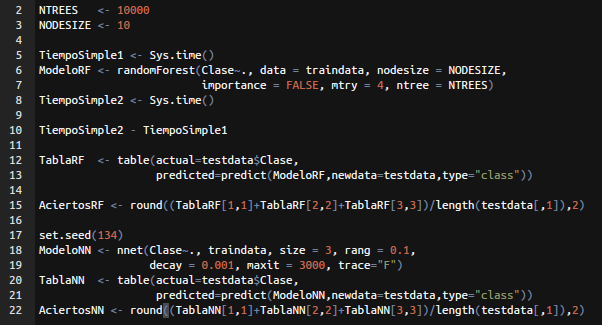
\includegraphics[width=1.25\linewidth]{images/Modelos.png}
  \caption{Red Neuronal y Random Forest }
\end{subfigure}%
\begin{subfigure}{.5\textwidth}
  \centering
  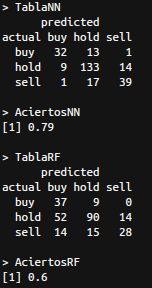
\includegraphics[width=.45\linewidth]{images/Tabla1.png}
  \caption{Tablas de resultados}
\end{subfigure}

\end{figure}



\end{frame}

% -- ----------------------------------------------------------------------------- -- %
% -- --------------------------- Kaggle como fuente de problemas en PAP Lamina (5) -- %
% -- ----------------------------------------------------------------------------- -- %

\begin{frame}{Kaggle \textit{The Home of Data Science}}

\begin{itemize}

  \item PonPare - Prediccion de cupones a comprar por clientes.
  \item Rossman - Prediccion de ventas de farmacias en Alemania.
  \item IMDB - An\'alisis de sentimiento en rese\~nas de peliculas.
  \item Bike Sharing - Predicci\'on de demanda de bicicletas.
  \item Otros...
\end{itemize}


\end{frame}

% -- ----------------------------------------------------------------------------- -- %
% -- ------------------------------------------- Propuesta de modelos I Zuri (1) -- %
% -- ----------------------------------------------------------------------------- -- %

\begin{frame}{Caso Rossman}

\begin{figure}[H]
\centering
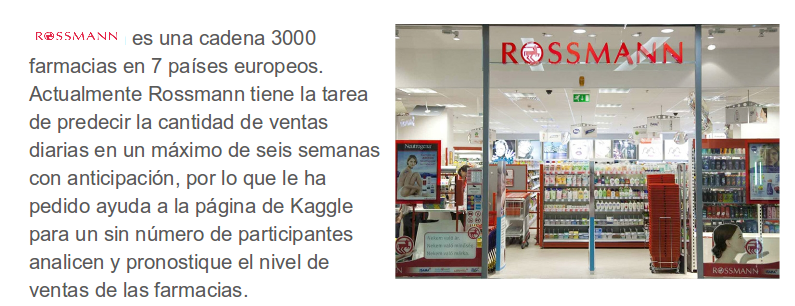
\includegraphics[scale=.36]{images/Zuri1.png}
\end{figure}


\end{frame}

% -- ----------------------------------------------------------------------------- -- %
% -- ------------------------- Clasificacion, Prediccion y desempeno I Zuri (2) -- %
% -- ----------------------------------------------------------------------------- -- %

\begin{frame}{Caso Rossman}

De acuerdo a los datos que se irán obteniendo a través de la metodología se
organizaran de la siguiente manera:

\vspace{.75cm}

\begin{enumerate}
  \item Descripción de variables
  \item Exploración de datos.
  \item Procedimiento de estimación (Logistic Regression, Tree, Random Forest
  \item Bagging, Boosting)
  \item Conclusiones de Análisis exploratorio
  \item Predicciones.
\end{enumerate}

\vspace{.75cm}

Variables: Id(tienda, Fecha), Costumer, SchoolHoliday, Promo, Store, Open,
Assortment (a,b,c), Promo2, Sales, StoreType, Competition Distance, Promo Interval


\end{frame}

% -- ----------------------------------------------------------------------------- -- %
% -- ------------------------ Clasificacion, Prediccion y desempeno II Zuri (3) -- %
% -- ----------------------------------------------------------------------------- -- %

\begin{frame}{Caso Rossman}

\begin{figure}[H]
\centering
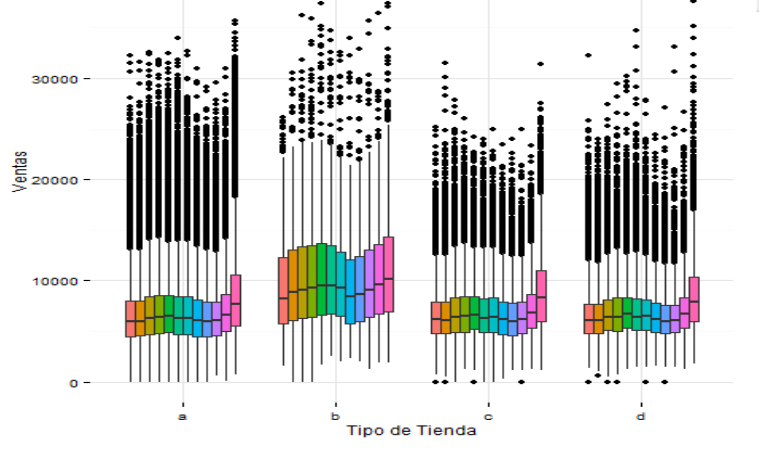
\includegraphics[scale=.35]{images/Zuri5.png}
\end{figure}

\end{frame}

% -- ----------------------------------------------------------------------------- -- %
% -- --------------------------------- Conclusiones y trabajo a futuro Zuri (4) -- %
% -- ----------------------------------------------------------------------------- -- %

\begin{frame}{Caso Rossman}

\begin{figure}[H]
\centering
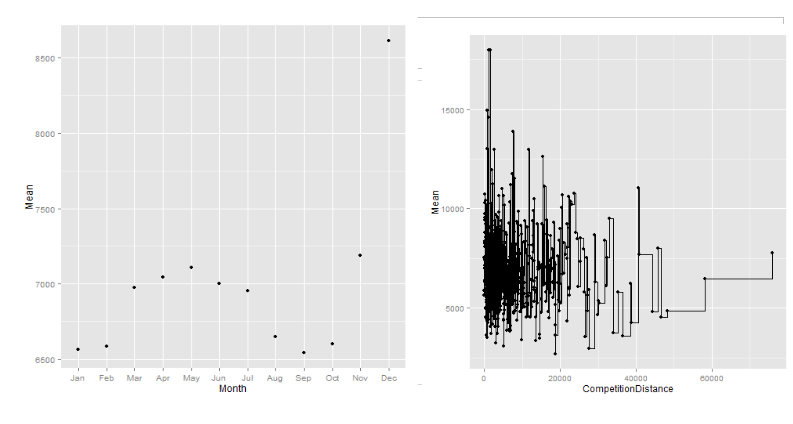
\includegraphics[scale=.35]{images/Zuri6.png}
\end{figure}

\end{frame}

% -- ----------------------------------------------------------------------------- -- %
% -- --------------------------------------------------------- Apoyo 1 Zuri (5) -- %
% -- ----------------------------------------------------------------------------- -- %

\begin{frame}{Conclusiones Caso Rossman}

\begin{figure}[H]
\centering
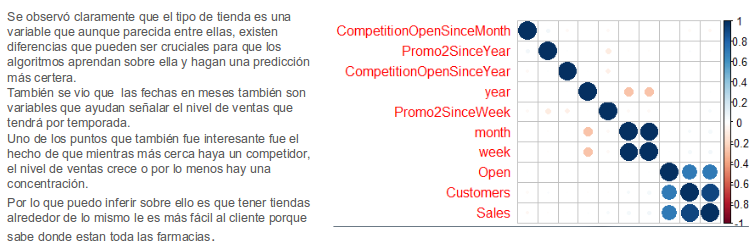
\includegraphics[scale=.42]{images/Zuri7.png}
\end{figure}

\textbf{Resultados de RMSPE}:

\begin{itemize}

  \item Regresión Lineal: 2735.217
  \item Tree: 2823.370
  \item Random Forest: 2488.109
  \item Bosting: 2196.695

\end{itemize}

\end{frame}

% -- ----------------------------------------------------------------------------- -- %
% -- --------------------------------------------------------- Apoyo 1 Zuri (7) -- %
% -- ----------------------------------------------------------------------------- -- %

\begin{frame}
\centering
\Huge Preguntas ?

\end{frame}


\end{document}
